\documentclass{article}

% if you need to pass options to natbib, use, e.g.,:
%     \PassOptionsToPackage{numbers, compress}{natbib}
% before loading neurips_2021

% ready for submission
\usepackage[preprint]{neurips_2023}

% to compile a preprint version, e.g.,, for submission to arXiv, add add the
% [preprint] option:
%     \usepackage[preprint]{neurips_2021}

% to compile a camera-ready version, add the [final] option, e.g.,:
%     \usepackage[final]{neurips_2021}

% to avoid loading the natbib package, add option nonatbib:
%    \usepackage[nonatbib]{neurips_2021}

\usepackage[utf8]{inputenc} % allow utf-8 input
\usepackage[T1]{fontenc}    % use 8-bit T1 fonts
\usepackage[colorlinks=true]{hyperref}       % hyperlinks
\usepackage{url}            % simple URL typesetting
\usepackage{booktabs}       % professional-quality tables
\usepackage{amsfonts}       % blackboard math symbols
\usepackage{nicefrac}       % compact symbols for 1/2, etc.
\usepackage{microtype}      % microtypography
\usepackage{xcolor}         % colors
\usepackage{graphicx}       % for images
\title{Decoding Eye-Catchiness: Exploring the\\Relationship Between Thumbnail Features\\and Viewer Metrics on YouTube}

% The \author macro works with any number of authors. There are two commands
% used to separate the names and addresses of multiple authors: \And and \AND.
%
% Using \And between authors leaves it to LaTeX to determine where to break the
% lines. Using \AND forces a line break at that point. So, if LaTeX puts 3 of 4
% authors names on the first line, and the last on the second line, try using
% \AND instead of \And before the third author name.

\author{%
  Lean Ting Jin\\
  Matrikelnummer 6956985\\
  \fontsize{8.5}{11}\texttt{ting-jin.lean@student.uni-tuebingen.de} \\
  \And
  Finn Springorum\\
  Matrikelnummer 6124977\\
  \fontsize{8.5}{11}\texttt{finn.springorum@student.uni-tuebingen.de} \\
  \And
  Christian Traxler\\
  Matrikelnummer 6969273\\
  \fontsize{8.5}{11}\texttt{christian.traxler@student.uni-tuebingen.de} \\
  \And
  Anna Chechenina\\
  Matrikelnummer 6987499\\
  \fontsize{8.5}{11}\texttt{anna.chechenina@student.uni-tuebingen.de} \\
}

\begin{document}

\maketitle

\begin{abstract}
Visually appealing YouTube thumbnails are believed to increase viewership and thus generate more income for creators. In this study, we investigate this hypothesis by analyzing the relationship between features associated with thumbnail eye-catchiness and the view count, based on 80,000 entertainment videos collected with the YouTube Data API \cite{youtubeapi}. We normalized view counts relative to subscriber counts and applied linear regression models to identify potential correlations. Our results suggest that videos with higher view count tend to have more eye-catching thumbnails. However, thumbnail features were insufficient to explain variations in view counts unaccounted for by subscriber counts. To our knowledge, this is the first study to examine the impact of thumbnail visual appeal on view counts.
\end{abstract}

\section{Introduction}
YouTube is the second most visited website in the world. In 2024, creators uploaded over 378 million hours of content to YouTube, and were paid more than 50 billion dollars in revenue~\cite{youtube-stats}. For YouTube creators, there is a significant financial incentive to maximize the views of their videos, whose promotion depends on the enigmatic YouTube algorithm. However, it is ultimately the user who decides in a split second whether a video is being watched. Thumbnails, the primary visual element presented to users, appear to play a crucial role in influencing user engagement and selection, as suggested by YouTube's official resources \cite{YouTubeThumbnail}. However, there appears to be no quantitative research on this topic in literature.

Quantifying the eye-catchiness of a thumbnail is inherently challenging. However, certain features, such as image color, saturation, and the presence of human faces, likely contribute to visual prominence. As a proxy for eye-catchiness, our study examines six thumbnail-derived features: hue, saturation, lightness, contrast, sharpness, and the number of faces. We hypothesize that more eye-catching thumbnails lead to higher video view counts.

\section{Methods}

\textbf{Data Collection.} We used the YouTube Data API \cite{youtubeapi} to collect video data from eight of YouTube's 15 categories: Comedy, Education, Entertainment, Gaming, How-to \& Style, News \& Politics, People \& Blogs, and Sports. These videos are primarily designed to appear in a user's feed and elicit a response, making them suitable for our thumbnail study.

Due to the limited number of videos that can be retrieved for a given query, the date range from January 1st, 2015 to the time of collection was divided into disjoint intervals, and 500 videos were requested for each interval. To prevent duplicates while respecting the daily API limit, we collected 2,500 videos from a designated category using a distinct singular generic keyword (e.g., most popular video games for the Gaming category), until the collection comprised precisely 10,000 unique videos from said category, yielding a dataset with a total of 80,000 unique videos.

\textbf{Video and Thumbnail Features.} For each video, we collected its thumbnail, view count, and subscriber count. From each thumbnail, we extracted six features: hue, saturation, lightness, contrast, sharpness, and the number of faces.

The hue is the angle of the mean color of the thumbnail in the HSV color space, with a range of 0 to 360 degrees. The saturation, lightness, and contrast follow their standard definitions as implemented in the OpenCV Python library \cite{opencv_library} (normalized to [0,1]). The sharpness is the log variance of the Laplacian of the grayscale image. The number of faces is the number of distinct faces in the thumbnail as predicted by the RetinaFace model implemented in the DeepFace library \cite{serengil2024lightface,serengil2020lightface}.


\textbf{Analysis.} We are interested the the relationship between the view count $N_i$ and the six features derived from the thumbnail $T_i$. However, as implied by intuition and a linear regression model (Fig.~\ref{fig:subscriber}), there is a strong positive Pearson correlation ($\rho=0.68$) between the view count of a video and the number of subscribers $S_i$ of its corresponding YouTube channel. To remove this effect and focus on variations in view count not explained by the subscriber count, we normalized the view count by applying linear regression (LR) models of the log view count against the log subscriber count for each category (log: base 10). The log-transformation ensures that the residuals are approximately homoscedastic and normally distributed, as the view and subscriber count distribution appears to be log-normal. This way, we obtained the residuals $R_{i} := \log(N_i) - \hat{\beta}_0^{(\gamma)} - \hat{\beta}_1^{(\gamma)} \log(S_i)$, with $\gamma \in \{1,..., 8\}$ corresponding to one of the eight categories that video $V_i$ belongs to. We refer to these residuals as "residual log view count" and use them as well as the non-normalized "log view count" for all models in the following analysis.


\begin{figure}[h]
  \begin{minipage}[t]{0.67\textwidth}
    \vspace{0pt}  % Removes top spacing
    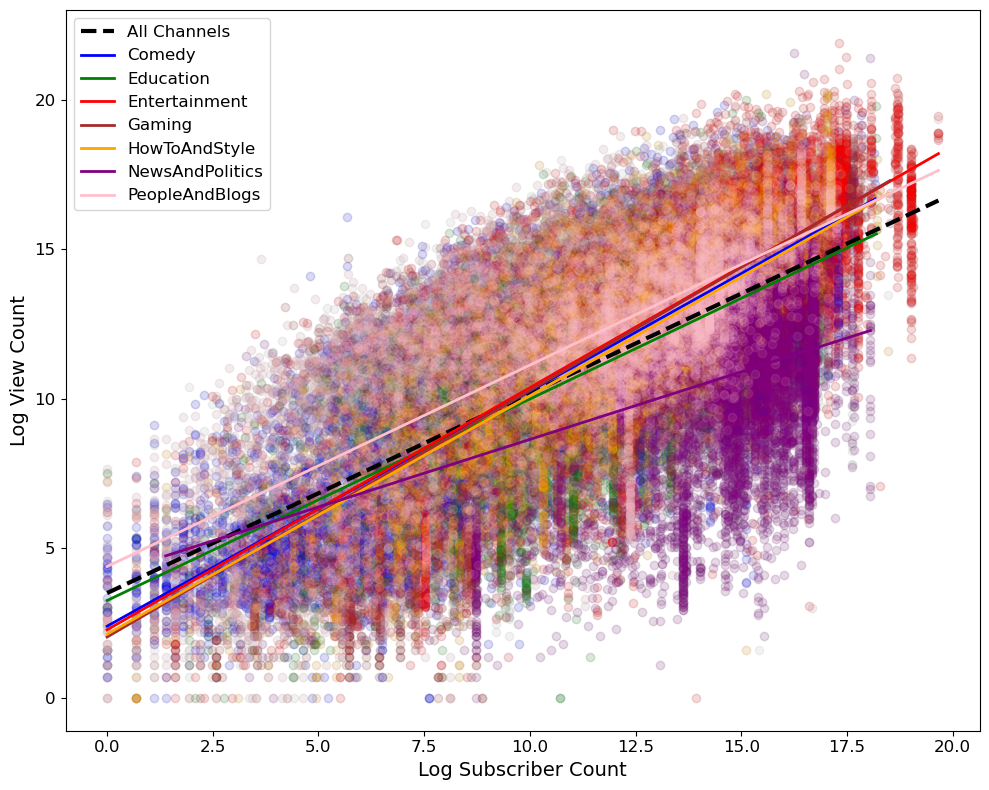
\includegraphics[width=\textwidth]{figs/subscriber.png}
  \end{minipage}%
  \hspace{0.05\textwidth}%
  \begin{minipage}[t]{0.27\textwidth}
    \vspace{0pt}  % Removes top spacing
    \caption{Linear regression (LR) of the log view count against the log subscriber count. The relationships are similar for all eight video categories. For the combined dataset, the relationship is $\widehat{\log(N_i)} = \hat{\beta}_0 + \hat{\beta}_1 \cdot \log(S_i)$, 95\% CI for $\beta_0$ is $[3.445, 3.571]$, 95\% CI for $\beta_1$ is $[0.663, 0.673]$, $R^2 = 0.467$.}
    \label{fig:subscriber}
  \end{minipage}
\end{figure}

Furthermore, the correlation between the six thumbnail features was investigated. There did not appear to be strong multicollinearity between features, except for the lightness-contrast correlation which was highly positive ($\rho=0.79$). A random forest regression model with 500 trees and three out of six features considered per split was applied to obtain some non-linear insights about the feature importance.

Moreover, a linear regression model was fitted to each continuous feature (saturation, lightness, contrast, sharpness). Meanwhile, the number of faces and the hue were treated as categorical features, and 95\% confidence intervals (CIs) of the log view count and residual log view count were computed for each category. The face count was divided into the categories 0, 1, 2, and 3+, with the last category comprising all videos with at least three detected faces on their thumbnail. The hue was divided into six bins corresponding to a 60-degree range.

Finally, both view counts were fitted against saturation, contrast, sharpness, and the number of faces in a multiple linear regression model. We removed the lightness feature due to the multicollinearity mentioned above, and the hue due to its unique and non-linear characteristics.

\section{Results}
We focus our analysis on the entire dataset with nearly 80,000 valid data points, since we did not observe significant differences between the eight video categories. For both the log view count and residual log view count, the feature importance results of the random forest model were similar for the five simple image features hue, saturation, lightness, contrast, and sharpness (around $0.19$), with slight variations between the categories, whereas the number of faces yielded a smaller importance of about $0.05$.

The linear regression models for the continuous features (Fig. \ref{fig:lr}) revealed a positive slope for the log view count against each feature, respectively, a smaller positive slope for the residual log view count against saturation, and even a negative slope for the relationship between normalized views and lightness, contrast, and sharpness, respectively. The 95\% confidence intervals for the face count and hue (Fig. \ref{fig:faces-and-hue}) also exhibited major differences between the log and residual log view counts: Whereas the log view count intervals for thumbnails with at least one face lay higher than and did not overlap with the interval for no faces, we could not observe this trend for the residual log view count. For the hue, however, the confidence intervals for both types of view counts with a mid-range average hue lay clearly above those of the 0-60 and 300-360 degree range.

\begin{figure}[h]


  \centering
  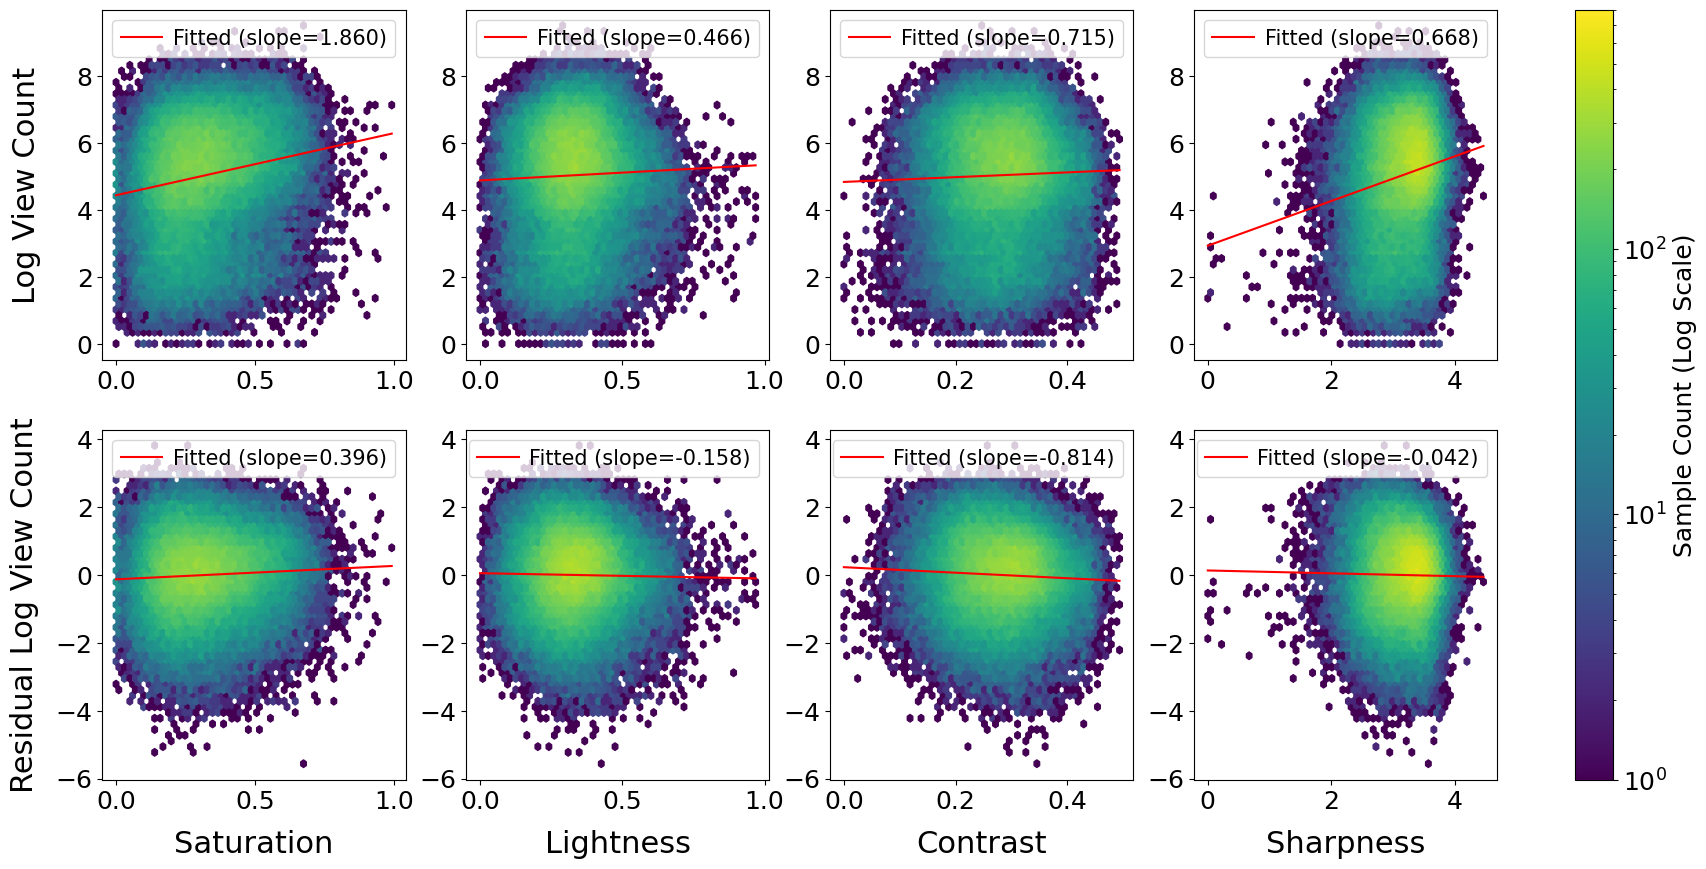
\includegraphics[width=\textwidth]{figs/lr.png}
  \caption{Linear regression results for the log view count (top) and the residual log view count (bottom) against the four features saturation, lightness, contrast, and sharpness, respectively, based on the entire dataset.}
  \label{fig:lr}
\end{figure}

\begin{figure}[h]
  \begin{minipage}[t]{0.67\textwidth}
    \vspace{0pt}  % Removes top spacing
    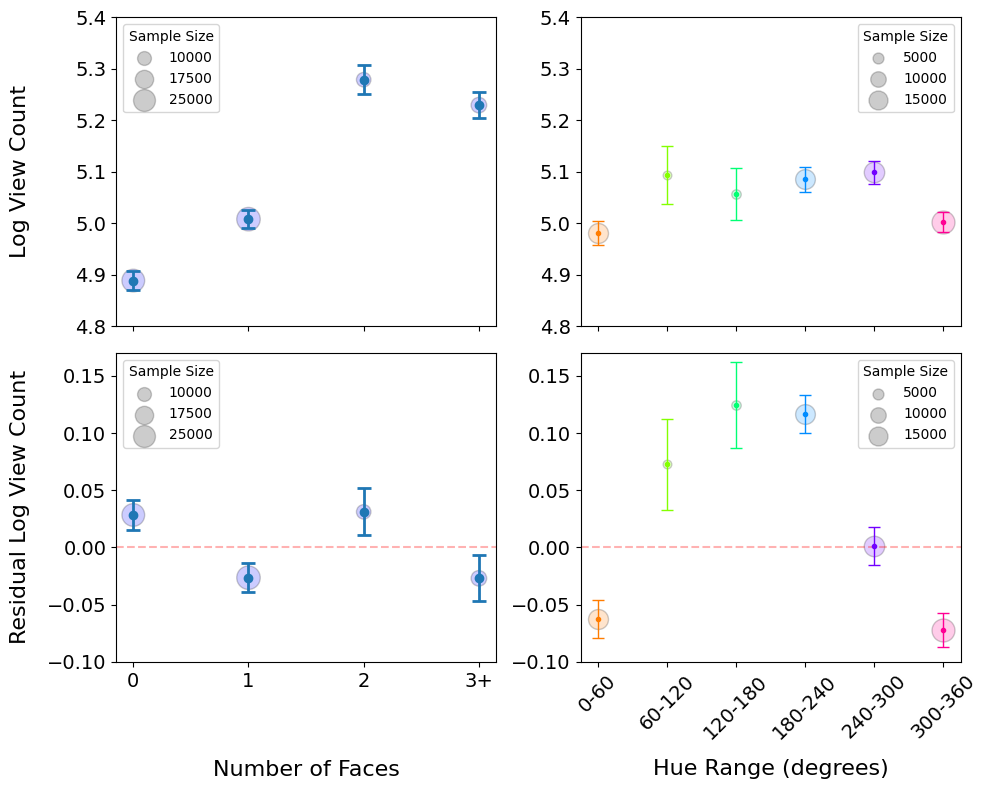
\includegraphics[width=\textwidth]{figs/faces-and-hue.png}
  \end{minipage}%
  \hspace{0.05\textwidth}%
  \begin{minipage}[t]{0.27\textwidth}
    \vspace{0pt}  % Removes top spacing
    \caption{95\% CIs of the log view count and residual log view count for each face and hue category, as previously defined. The color of each hue boxplot was chosen according to the central hue of the corresponding bin.}
    \label{fig:faces-and-hue}
  \end{minipage}
\end{figure}

\begin{table}[h]
\centering
\begin{tabular}{lrrrr}
\toprule
& \multicolumn{2}{c}{Non-normalized} & \multicolumn{2}{c}{Normalized} \\
\cmidrule(lr){2-3} \cmidrule(lr){4-5}
Feature & 95\% CI & $p$-value & 95\% CI & $p$-value \\
\midrule
Saturation & [1.482, 1.627] & $<10^{-308}$ & [0.362, 0.470] & $<10^{-308}$ \\

Contrast & [-1.587, -1.236] & $<10^{-308}$ & [-1.043, -0.780] & $<10^{-41}$ \\
Sharpness & [0.637, 0.699] & $<10^{-308}$ & [-0.011, 0.036] & 0.294 \\
Number of faces & [0.012, 0.020] & $<10^{-13}$ & [-0.013, -0.006] & $<10^{-8}$ \\
\bottomrule
\end{tabular}
\vspace{\baselineskip}
\caption{95\% coefficient CI and $p$-value for each feature in the two multiple linear regression models. $R^2 = 0.055$ (log view count) and $R^2 = 0.006$ (residual log view count).}
\label{tab:regression}
\end{table}

For the multiple linear regression model (Tab.~\ref{tab:regression}) based on the four features saturation, contrast, sharpness, and number of faces, we obtained $p$-values negligibly close to zero for the overall model. For the non-normalized view count, all $p$-values for the different features were almost zero, and all coefficients except for the contrast coefficient were positive. For the normalized view count, the $p$-value for sharpness was $0.294$, the others were almost zero as well, and the coefficients were mostly negative or close to zero, except for the saturation coefficient.

\section{Discussion/Limitations}
\textbf{Findings.} The near-zero $p$-values of our multiple linear regression results indicate a significant relationship between multiple features we associate with the eye-catchiness of a thumbnail and the view count of the corresponding video. However, one must distinguish between the non-normalized and the normalized version of the view count. For the former one, we observed positive slopes in the single regression models, and a significant difference between videos with and without faces on their thumbnails. Although these observations support our hypothesis, the causality remains unclear, since these findings could also imply that more successful channels produce more eye-catching thumbnails, but obtain more views due to other features unrelated to eye-catchiness. Most importantly, the clear correlation with the subscriber count must be addressed. After normalizing the view count, most of our regression plots no longer showed positive relationships. This suggests that the eye-catchiness, as defined by us, is likely insufficient to explain the variations in view count for a fixed number of subscribers. Only the saturation feature coefficients were always positive, which may indicate that saturation is the most important feature to optimize as a YouTube creator. The random forest model did not provide valuable information either, since the five simple image features were relatively similar in terms of predictive power, only the face count showed a much lower feature importance which might be due to its discrete and thus limited nature. Interestingly, the analysis for the hue was consistent across non-normalized and normalized view counts, indicating that thumbnails with predominantly green and blue colors might yield more views on average compared to reddish ones.

\textbf{Other limitations.} There were some inherent limitations of the YouTube Data API. First, the 15 video categories offered are somewhat overlapping and vague, being user-defined or automatically generated. The API also does not give access to the average view duration of a video, which, like subscriber count, is another important factor to be accounted for. In addition, despite our dataset being reasonably large, it cannot be fully representative of all YouTube videos, since the algorithm decided which videos we were able to collect, and they had a bias towards either popular or recent videos.

\textbf{Text detection.}

\section{Statement of Contributions}

%\emph{Here is an example:}

Chase and Finn set up the API scripts, performed the correlation and regression analysis, and created the plots. Christian wrote API scripts to collect the subscriber counts for our dataset. Anna implemented and analyzed the text detection methods and models. All members of the group contributed to collecting the dataset and writing the report.
% XX performed the correlation analysis, organized the data and code for the processing of dataset1 and subdataset2, and created the scatter plot. 
% YY created the random forest regression model, performed the data cleaning for the xyz analysis / xyz database, and created the bar charts to display the regression results. 
% ZZ researched and collected the raw data, restructured the pipeline for the data analysis, and proof-read the draft for the final report. 
% AA performed the data cleaning for dataset1, and performed the Ridge and Lasso regularization. 
% All members of the group contributed to writing the report.



\bibliographystyle{unsrt}%Used BibTeX style is unsrt
\bibliography{bibliography}

\end{document}